
\chapter{HASIL DAN PEMBAHASAN}


%Jelaskan Tentang Proses Filter spasial 
\section{Filter Spasial Linear}
\blindtext
\begin{afigure}
    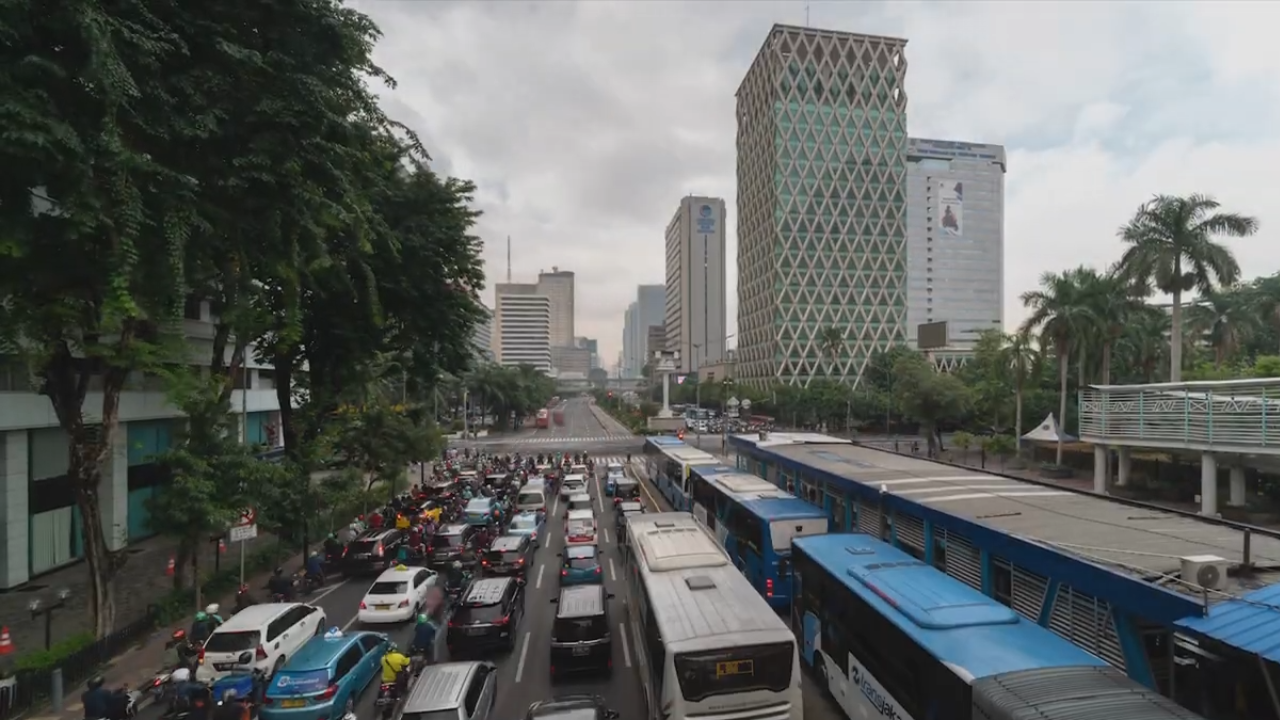
\includegraphics[width=\linewidth, center]{images/input-image/input1.png}
    \caption{Contoh Frame (Citra Input).}
    \label{fig:input-image-rgb}
\end{afigure}
\blindtext
\begin{afigure}
    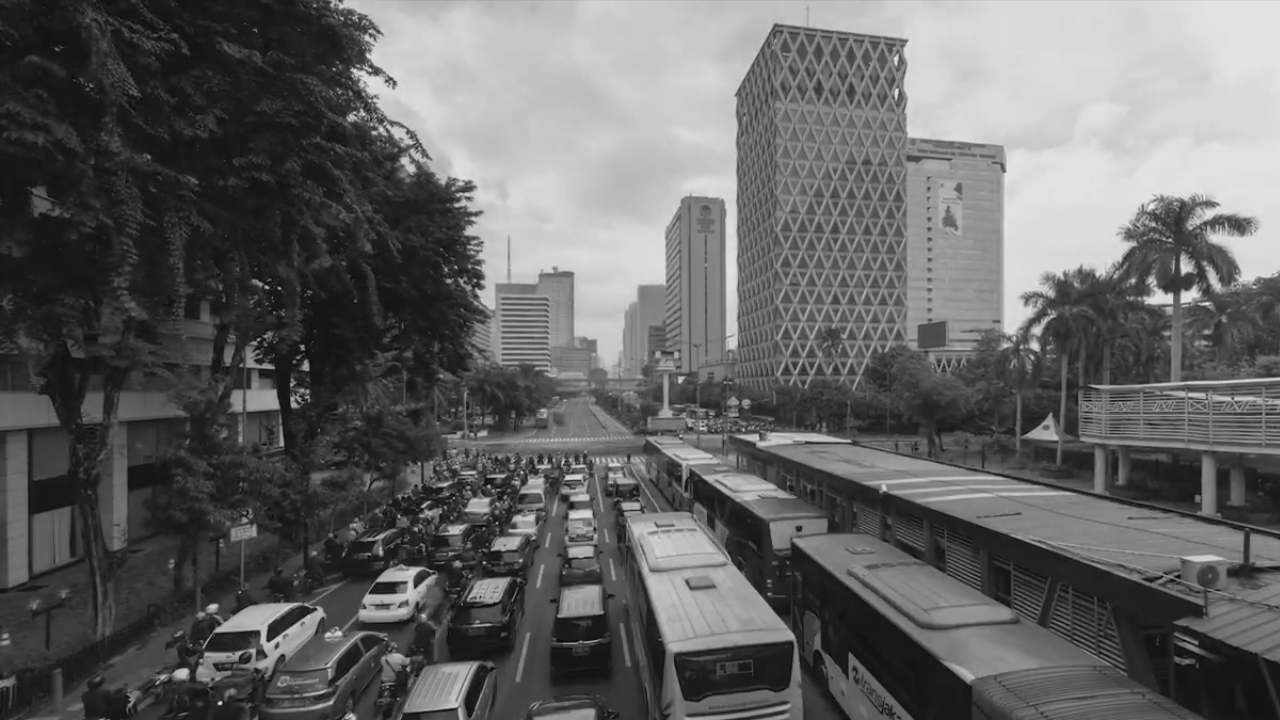
\includegraphics[width=\linewidth, center]{images/output-image/input1-grayscale.png}
    \caption{Contoh Frame Grayscale.}
    \label{fig:input-grayscale}
\end{afigure}

\subsection{Average Blur}
\blindtext
\begin{afigure}
    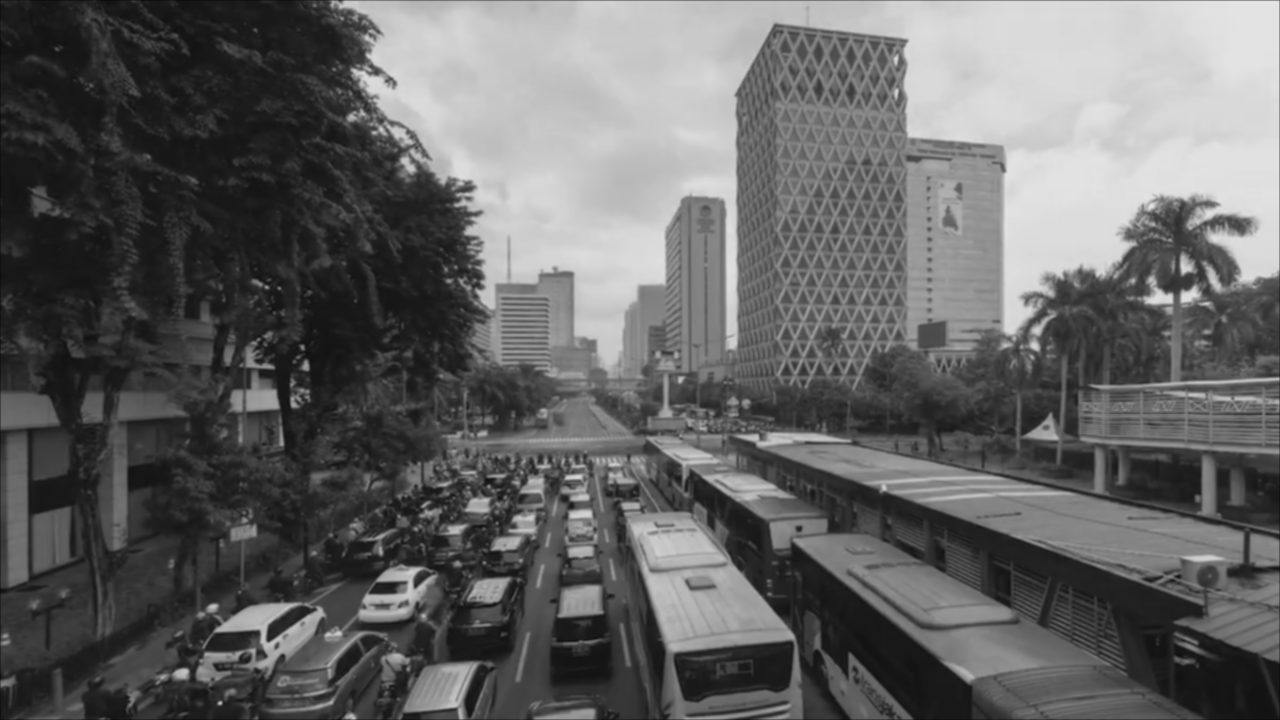
\includegraphics[width=\linewidth, center]{images/output-image/input1-averageblur.png}
    \caption{Hasil filter Average Blur.}
    \label{fig:output-averageblur}
\end{afigure}

\subsection{Gaussian Blur}
\blindtext
\begin{afigure}
    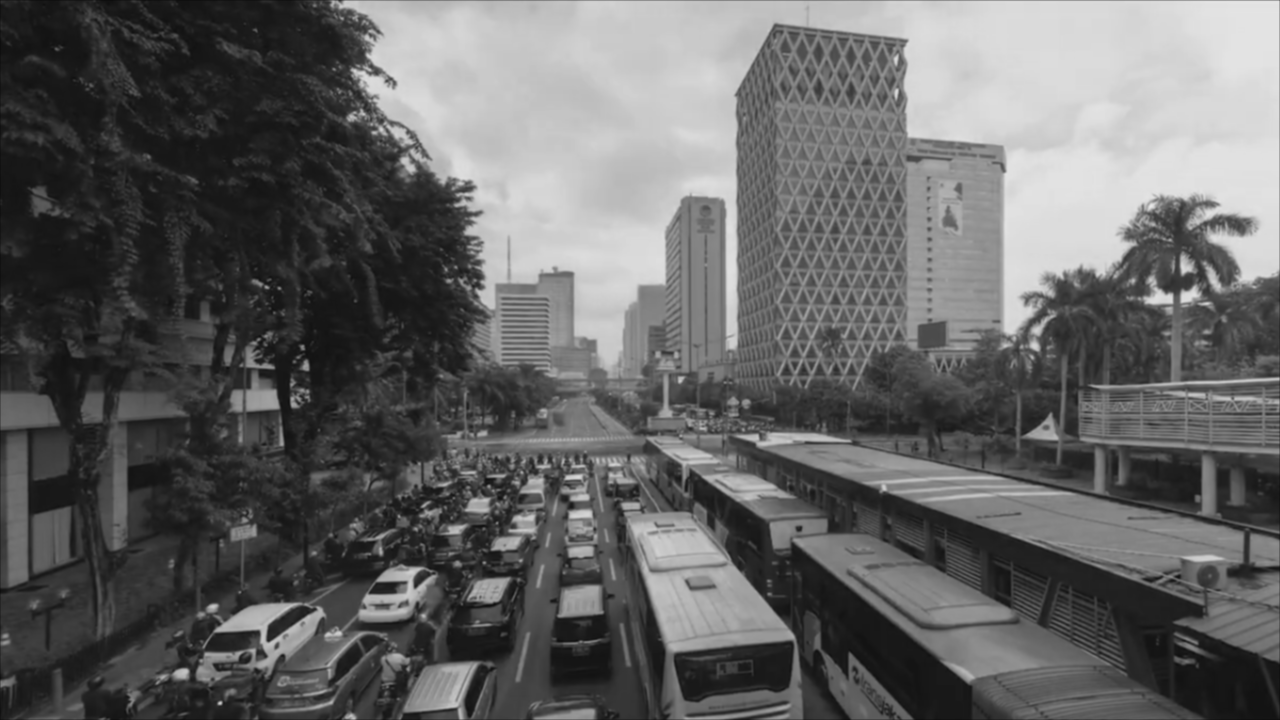
\includegraphics[width=\linewidth, center]{images/output-image/input1-gaussianblur.png}
    \caption{Hasil filter Gaussian Blur.}
    \label{fig:output-gaussianblur}
\end{afigure}

\subsection{Laplacian}
\blindtext
\begin{afigure}
    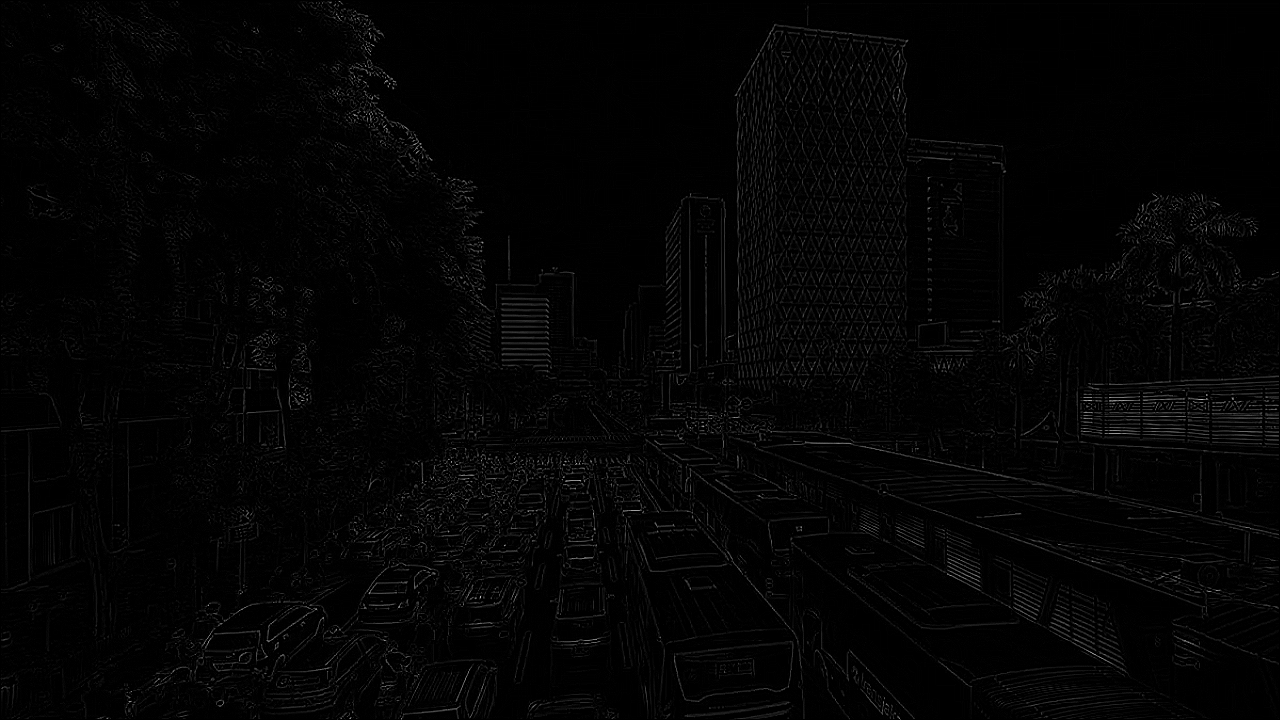
\includegraphics[width=\linewidth, center]{images/output-image/input1-laplacian.png}
    \caption{Hasil filter Laplacian.}
    \label{fig:output-laplacian}
\end{afigure}

\subsection{Sharpening}
\blindtext
\begin{afigure}
    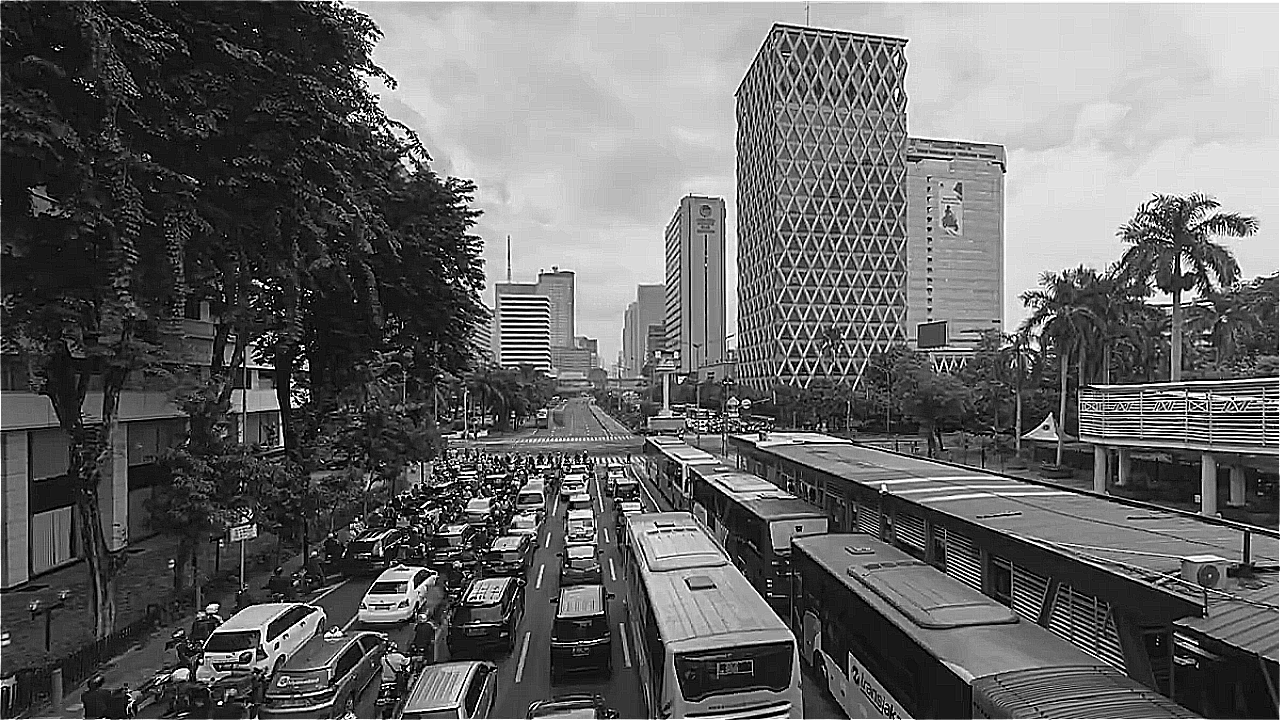
\includegraphics[width=\linewidth, center]{images/output-image/input1-sharpen.png}
    \caption{Hasil filter Sharpening.}
    \label{fig:output-sharpen}
\end{afigure}

\subsection{Sobel Horizontal}
% \blindtext
\begin{afigure}
    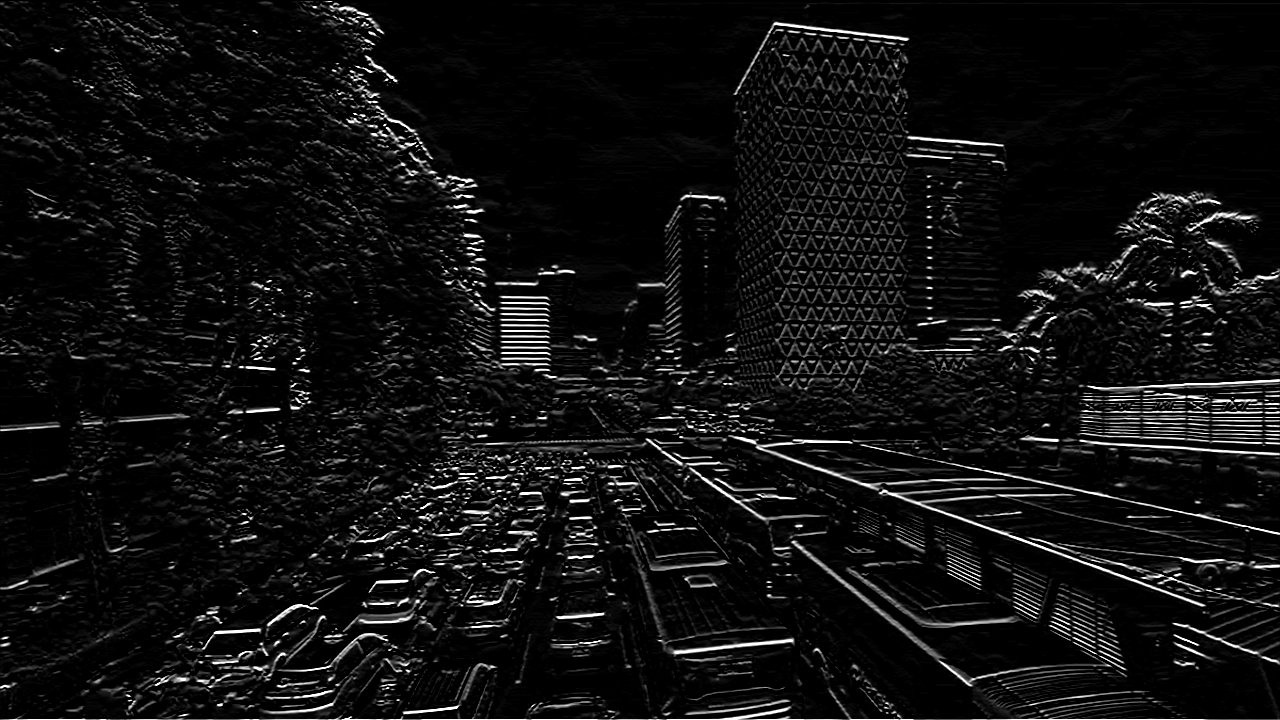
\includegraphics[width=\linewidth, center]{images/output-image/input1-sobelhor.png}
    \caption{Hasil filter Sobel Horizontal.}
    \label{fig:output-sobelhor}
\end{afigure}

\subsection{Sobel Vertical}
\blindtext
\begin{afigure}
    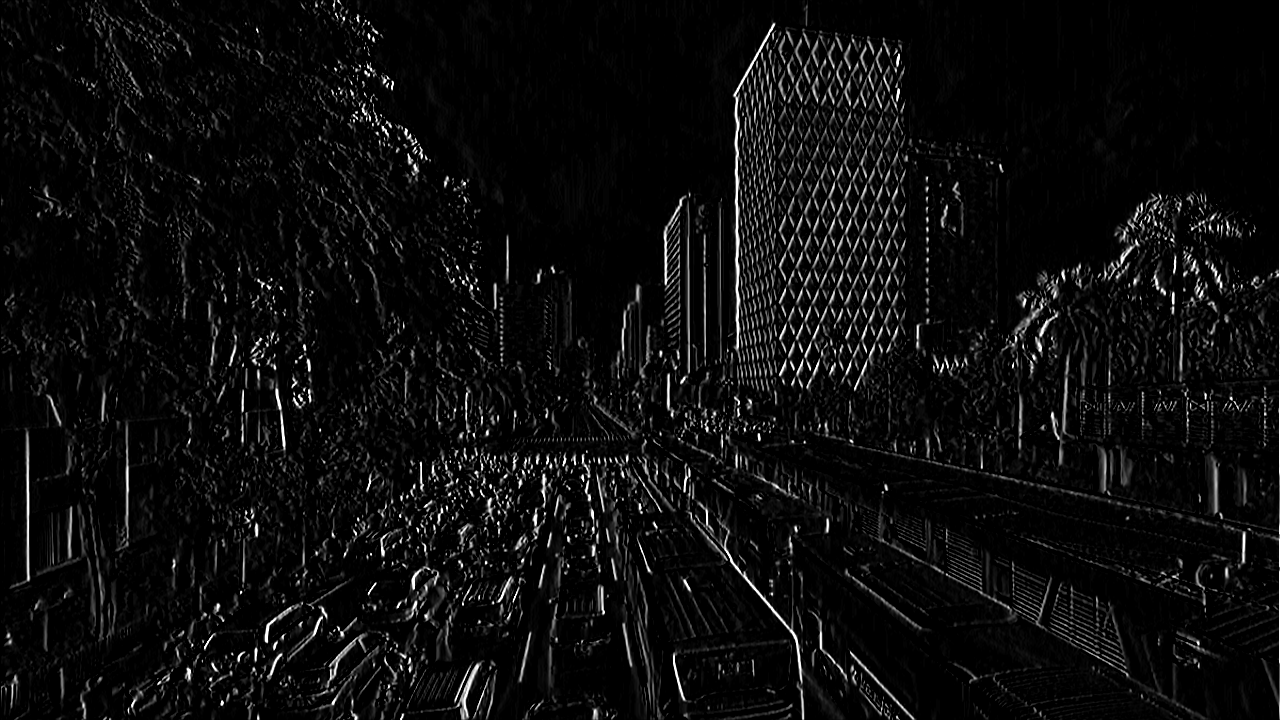
\includegraphics[width=\linewidth, center]{images/output-image/input1-sobelver.png}
    \caption{Hasil filter Sobel Vertical.}
    \label{fig:output-sobelver}
\end{afigure}

% Jelaskan Proses Implementasi 
\section{Implementasi pada FPGA Development Board}
\blindtext
\subsection{Representasi Video Stream sebagai Citra Digital}
\subsection{Konversi Frame menjadi Grayscale}
\subsection{Penerapan Filter Spasial}
\subsection{Analisis Kinerja}


% Jelaskan Hasil
\section{Analisis Kinerja}
\subsection{Frame Rate (FPS)}

\begin{atable}
    \caption{Perbandingan waktu komputasi}
    \label{table:hasil-fps}
    \csvreader[
        head to column names,
        tabular=lcc,
        before table=\rowcolors{2}{gray!15}{gray!30},
        table head= \rowcolor{gray!50!black} 
            \color{white} Filter & 
            \color{white} Tanpa FPGA & 
            \color{white} Dengan FPGA \\]
        {tables/hasil-fps.csv}
        {filter=\filter, tanpafpga=\tanpafpga, denganfpga=\denganfpga}
        {\filter & \tanpafpga & \denganfpga }
\end{atable}

\subsubsection{Prosesor ARM}
\subsubsection{FPGA}

\subsection{Penggunaan CPU}
\blindtext
\subsubsection{Prosesor ARM}
\subsubsection{FPGA}

\subsection{Penggunaan Memory}
\blindtext
\subsubsection{Prosesor ARM}
\subsubsection{FPGA}

\subsection{Resident Memory (RES)}
\blindtext
\subsubsection{Prosesor ARM}
\subsubsection{FPGA}

\subsection{Shared Memory (SHR)}
\blindtext
\subsubsection{Prosesor ARM}
\subsubsection{FPGA}

\subsection{Virtual Memory (VIRT)}
\blindtext
\subsubsection{Prosesor ARM}
\subsubsection{FPGA}